%=======================================================================
% cap1_introduccion.tex
%=======================================================================

\section{Motivación y contexto}\label{sec:motivacion}

La biodiversidad sostiene los procesos que hacen posible la vida humana:
regula el clima, mantiene el equilibrio de los ecosistemas y sustenta las
actividades productivas. La pérdida de diversidad biológica reduce la
productividad y la estabilidad de los ecosistemas y compromete los servicios
que estos proveen a la sociedad. A escala global, la Plataforma
Intergubernamental sobre Biodiversidad y Servicios Ecosistémicos estima que
cerca de un millón de especies se encuentran en riesgo de extinción como
consecuencia de actividades humanas, con tasas de declive sin precedentes en
la historia reciente \citep{ipbes2019}.

Chile no es ajeno a esta crisis. El listado oficial del Reglamento de
Clasificación de Especies (RCE), actualizado a marzo de 2026 tras su
vigésimo proceso, registra \num{1591} especies clasificadas, de las cuales
208 se encuentran En Peligro Crítico, 446 En Peligro y 340 Vulnerables. A
ellas se suman 20 especies Extintas o Extintas en Estado Silvestre
\citep{mma2026rce}. El \SI{62,5}{\percent} de las especies clasificadas
está en alguna categoría de amenaza, proporción que ya superaba el
\SI{60}{\percent} en el Reporte del Estado del Medio Ambiente de 2021
\citep{mma2021rema}. Es una señal de alerta para la conservación del
patrimonio natural. La zona central del país forma parte del
\textit{hotspot} de biodiversidad ``Chile central'' (bosques lluviosos
invernales y valdivianos), una de las 25 regiones del planeta con mayor
concentración de especies endémicas y mayor pérdida de hábitat, que conserva
solo alrededor del \SI{30}{\percent} de su vegetación original
\citep{myers2000hotspots}.

Las aves son sensibles a los cambios del hábitat, tienen amplia
distribución y son relativamente fáciles de detectar. Por eso se utilizan
como bioindicadores del estado de los ecosistemas: la mayoría de los índices
de biodiversidad con que se evalúa el cumplimiento de acuerdos
internacionales se construye sobre datos de aves \citep{fraixedas2020birds}. En Chile, la Estrategia Nacional de Conservación
de Aves las define como ``especies centinelas'' cuya presencia se relaciona
con ecosistemas más diversos, aguas no contaminadas y baja presencia de
especies exóticas invasoras \citep{mma2022enca}. El mismo instrumento
reconoce que el monitoreo de aves a escala nacional es caro en dinero y en
tiempo, que depende de especialistas y que la escasez de financiamiento es,
según los ornitólogos del país, la principal barrera al avance de la
disciplina.

El caso de las aves ilustra la magnitud del problema. Chile alberga 528
especies de aves nativas, el \SI{5}{\percent} de las aves del mundo, de las
cuales 322 se reproducen en el país. Doce son endémicas: nueve del territorio continental
y tres del archipiélago de Juan Fernández \citep{barros2015lista,
mma2022enca}. Según la misma Estrategia, hasta el proceso 17 del RCE se había
evaluado el estado de conservación de 114 especies y tres subespecies de aves.
De ellas, 59 resultaron amenazadas (En Peligro Crítico, En Peligro o
Vulnerable), 25 Casi Amenazadas y dos con Datos Insuficientes. Los procesos
posteriores han seguido incorporando aves: el listado oficial vigente
incluye 147 especies de aves clasificadas por el RCE, de las cuales 7 se
encuentran En Peligro Crítico, 31 En Peligro y 33 Vulnerables, es decir, 71
especies amenazadas (\SI{48}{\percent}), además de 32 Casi Amenazadas
\citep{mma2026rce}. Detectar oportunamente cambios en estas poblaciones exige
herramientas de monitoreo más eficientes y de mayor cobertura espacial y
temporal.

Paralelamente, existe un volumen creciente de datos de ciencia ciudadana y de
sensores remotos que permanece en gran parte subutilizado para el monitoreo
automático. eBird, el mayor proyecto de ciencia ciudadana del mundo, superó
en 2025 los dos mil millones de observaciones de aves, aportadas por 1,1
millones de observadores en 253 países \citep{sullivan2014ebird,
ebird2025billion}. Xeno-canto reúne más de \num{750000} grabaciones de cantos
de más de \num{10000} especies \citep{vellinga2015xenocanto, hamer2023birb}.
iNaturalist y GBIF concentran millones de fotografías geolocalizadas
\citep{vanhorn2018inaturalist}. Misiones satelitales como Sentinel-2
entregan imágenes multiespectrales de \SI{10}{\metre} de resolución con
revisita de pocos días \citep{drusch2012sentinel2}. En Chile esta
información ya ha demostrado su valor. El Atlas de las Aves Nidificantes de
Chile se construyó a partir de más de \num{675000} registros de eBird
aportados por \num{1815} personas \citep{medrano2018atlas}. La propia
Estrategia Nacional identifica a la ciencia ciudadana como una herramienta
central para un futuro sistema nacional de monitoreo. Este trabajo busca
aprovechar esa información con aprendizaje profundo e integrar varias
modalidades en un sistema único de apoyo a la conservación de la avifauna
chilena.

%-----------------------------------------------------------------------
\section{Descripción general del problema}\label{sec:problema}

El sistema aborda dos problemas complementarios, ilustrados en la
\figref{fig:arquitectura}. El primero es la \textbf{identificación multimodal
de especies}: dada una grabación de canto y/o una fotografía, determinar
automáticamente la especie de ave correspondiente entre un conjunto cerrado de
especies chilenas. Se trata de un problema de clasificación \textit{fine-grained} (``de grano
fino''): a diferencia de distinguir categorías muy distintas entre sí, como
un ave de un automóvil, aquí todas las clases son subcategorías de una misma
familia, aves, que comparten la estructura general y se diferencian por
detalles sutiles del plumaje, la silueta o el canto
\citep{wei2022finegrained}. El segundo es el \textbf{modelado de la
distribución espaciotemporal}: estimar la probabilidad de presencia de una
especie en función de la ubicación geográfica, la época del año y variables
ambientales, a partir de registros de solo presencia provenientes de ciencia
ciudadana \citep{elith2009sdm}.

Ambos problemas se abordan con aprendizaje automático. Para la identificación, el audio se representa como espectrogramas mel
procesados por redes convolucionales y/o por el \textit{Audio Spectrogram
Transformer}. Las imágenes se procesan mediante \textit{transfer learning}
con arquitecturas como EfficientNet y/o ViT. Las predicciones de ambas
modalidades se combinan por \textit{late fusion}, es decir, ponderando las
probabilidades que entrega cada clasificador, lo que permite operar también
cuando solo una modalidad está disponible. Otras estrategias de fusión
(\textit{early} e \textit{intermediate fusion}) se evalúan para comparar
metodologías. Para la distribución, se entrenan modelos de distribución de
especies (SDM) basados en redes neuronales y en Random Forest que integran
registros de avistamientos de eBird e iNaturalist (vía GBIF) con covariables
climáticas, índices de vegetación satelitales y elevación calculados en
Google Earth Engine. Estos modelos se comparan con MaxEnt
\citep{phillips2006maxent}, el método de referencia en ecología.

Tres preguntas guían el trabajo: si un sistema multimodal identifica mejor
que los clasificadores de una sola modalidad y que un modelo de IA generativa,
si un modelo de distribución basado en aprendizaje automático supera a MaxEnt,
y cómo afecta la escasez de datos a las especies amenazadas. Se formalizan,
junto con los objetivos, en la \secref{sec:objetivos}.

El alcance se limita a Chile continental, con foco en especies endémicas y en
estado de conservación Vulnerable, En Peligro o En Peligro Crítico según el
RCE del Ministerio del Medio Ambiente. Se excluyen las islas oceánicas
(Juan Fernández, Rapa Nui, Desventuradas) por su avifauna diferenciada y por
la escasez de registros disponibles.

\begin{figure}[!htb]
  \centering
  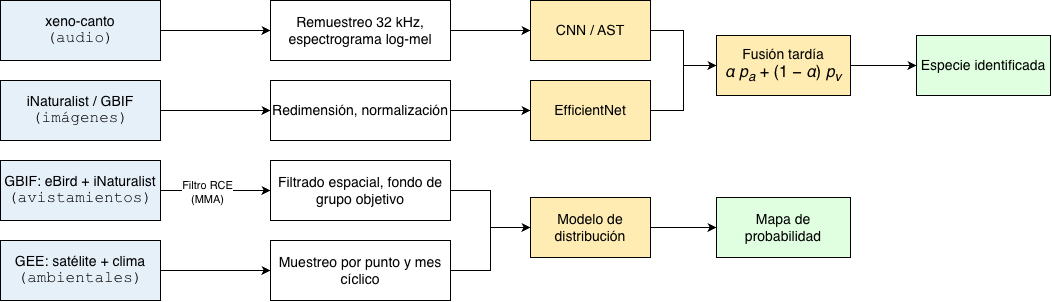
\includegraphics[width=\textwidth]{fig_arquitectura.png}
  \caption{Arquitectura general del sistema: las fuentes de datos (azul) se
  preprocesan (blanco) y alimentan los modelos (amarillo), dos clasificadores
  de audio e imagen cuyas probabilidades se combinan por \textit{late
  fusion}, y un modelo de distribución espaciotemporal comparado con MaxEnt;
  en verde, las salidas. El listado del RCE define las especies objetivo.}
  \label{fig:arquitectura}
\end{figure}

%-----------------------------------------------------------------------
\section{Contribuciones}\label{sec:contribuciones}

Los enfoques previos para la identificación de aves suelen abordar una sola
modalidad. En audio, BirdNET \citep{kahl2021birdnet} es hoy la herramienta
más difundida, pero una evaluación global reciente muestra que su capacidad
predictiva es máxima en Norteamérica, Oceanía y Europa y solo moderada en
Centro y Sudamérica, con \textit{recall} que oscila entre 0,24 y 0,52 según
el continente, lo que refleja diferencias en la cobertura de especies de sus
datos de entrenamiento \citep{funosas2026birdnet}. En imagen, los
clasificadores \textit{fine-grained} se han desarrollado sobre conjuntos como
CUB-200-2011 \citep{wah2011cub} e iNaturalist, dominados por avifaunas del
hemisferio norte. La combinación de audio e imagen para aves ha sido
explorada solo recientemente y con especies norteamericanas
\citep{vanhorn2022ssw60}. En el modelado de distribución,
MaxEnt sigue siendo el método de referencia en ecología y uno de los de
mejor desempeño con datos de solo presencia \citep{elith2011maxent,
valavi2022benchmark}, mientras que los SDM basados en aprendizaje profundo
son un área emergente \citep{deneu2021cnn, cole2023sinr}. No se identificó en
la literatura un sistema integrado que combine identificación multimodal y
modelado de distribución para la avifauna chilena.

Las principales contribuciones de este trabajo son:

\begin{enumerate}[leftmargin=*, itemsep=2pt]
  \item Un \textbf{clasificador multimodal} de 55 especies de aves chilenas
        (53 en ambas modalidades), con \textit{late fusion} de audio e imagen,
        evaluado frente a clasificadores de una sola modalidad (solo audio o
        solo imagen), a clasificadores sobre \textit{frozen embeddings} y a un
        modelo de IA generativa multimodal.
  \item Un \textbf{modelo de distribución espaciotemporal} que integra
        avistamientos, clima, índices de vegetación y elevación, comparado con
        MaxEnt mediante redes neuronales, Random Forest y gradient boosting,
        con partición aleatoria y validación cruzada espacial, incluida una
        evaluación del aporte de los parches de cobertura de suelo y los
        \textit{embeddings} de imágenes satelitales.
  \item Un \textbf{repositorio reproducible} que integra fuentes de datos
        heterogéneas, con un pipeline documentado y reanudable de descarga,
        normalización, partición, entrenamiento y evaluación, y un prototipo
        que integra los modelos, reutilizable para otras especies o regiones.
  \item Una \textbf{caracterización cuantitativa de la escasez de datos} de
        audio, imagen y avistamientos para las especies amenazadas de Chile,
        hallazgo que condiciona el diseño de cualquier sistema de monitoreo
        orientado a la conservación, junto con la evidencia de qué
        estrategias la mitigan en cada modalidad.
\end{enumerate}

\subsection{Contribuciones en términos de precisión}

\begin{enumerate}[leftmargin=*, itemsep=2pt]
  \item El clasificador multimodal supera a los clasificadores de una sola
        modalidad y a un modelo de IA generativa multimodal, y alcanza 0,945
        de \textit{accuracy} sobre 53 especies, por sobre la meta
        del \SI{85}{\percent}, en línea con lo observado en el
        \textit{benchmark} audiovisual SSW60, donde la fusión de modalidades
        supera a cada modalidad por separado. Las ramas de audio (0,858 y
        0,870) e imagen (0,848) cumplen o rozan la meta por sí solas.
  \item El modelo de distribución basado en Random Forest supera a
        MaxEnt en AUC-ROC con partición aleatoria (0,884 frente a 0,863), pero
        no al extrapolar a bloques espaciales no vistos, donde todos los
        modelos empatan. La red neuronal propuesta inicialmente no lo supera
        en ningún protocolo, un resultado negativo que se documenta con
        evidencia y que matiza la expectativa de la literatura sobre SDM
        profundos.
\end{enumerate}

\subsection{Contribuciones en términos de eficacia}

\begin{enumerate}[leftmargin=*, itemsep=2pt]
  \item El sistema automatiza la identificación y el monitoreo, reduce la
        dependencia de inspección experta en terreno y permite procesar
        grandes volúmenes de registros que hoy no pueden revisarse manualmente.
  \item El uso exclusivo de fuentes públicas y de cómputo en la nube (Google
        Earth Engine para el muestreo de las covariables ambientales) elimina
        el costo de adquisición de datos y evita la descarga y el almacenamiento
        local de imágenes satelitales.
  \item Los modelos de distribución permiten priorizar zonas de monitoreo y
        apoyar la planificación territorial para la conservación, en línea con
        las acciones de investigación y monitoreo que promueve la Estrategia
        Nacional de Conservación de Aves.
\end{enumerate}

%-----------------------------------------------------------------------
\section{Estructura del trabajo}\label{sec:estructura}

El resto del documento se organiza como sigue. El \capref{cap:relacionado}
revisa el trabajo relacionado en tres áreas, avanzando desde lo general a lo
específico: identificación bioacústica con aprendizaje profundo,
clasificación de aves por imagen (incluida la fusión multimodal) y modelos
de distribución de especies. El capítulo cierra con una tabla comparativa y la
identificación de la brecha de la literatura. El \capref{cap:teoria} presenta
las bases teóricas: la pregunta de investigación con el objetivo general y
los objetivos específicos, la formalización matemática de los problemas de
clasificación, \textit{late fusion} y distribución, las herramientas, metodologías y
métricas seleccionadas, sus virtudes en el contexto del problema y los
efectos positivos esperados. El \capref{cap:datos} documenta el
levantamiento de datos: la construcción de los corpus de audio, imagen y
avistamientos con sus covariables, los hallazgos derivados de la escasez de
datos en especies amenazadas y las desviaciones respecto del plan. El
\capref{cap:resultados} presenta los resultados de los clasificadores de
audio e imagen, de la fusión multimodal, de los \textit{baselines} de
referencia y del modelo de distribución frente a MaxEnt, junto con el
prototipo integrado y el costo computacional. El \capref{cap:conclusiones}
responde las preguntas de investigación, discute los hallazgos, declara las limitaciones y los aspectos éticos, recoge las lecciones
aprendidas y propone el trabajo futuro.
